
\documentclass[11pt]{article}
\usepackage[hmargin=1in,vmargin=1in]{geometry}
\usepackage{xcolor}
\usepackage{mdframed}
\newmdenv[linecolor=blue,backgroundcolor=blue!10]{mybox}
\usepackage{tikz}
\usepackage{adjustbox}

\usetikzlibrary{shapes,arrows}
\usepackage{enumitem}
\usepackage{amsmath,amssymb,amsfonts,url,sectsty,framed,tcolorbox,framed}
\newcommand{\pf}{{\bf Proof: }}
\newtheorem{theorem}{Theorem}
\newtheorem{lemma}{Lemma}
\newtheorem{proposition}{Proposition}
\newtheorem{definition}{Definition}
\newtheorem{remark}{Remark}
\newcommand{\qed}{\hfill \rule{2mm}{2mm}}
\usepackage{enumitem}



\begin{document}
%%%%%%%%%%%%%%%%%%%%%%%%%%%%%%%%%%%%%%%%%%%%%%%%%%%%%%%%%%%%%%%%%%%%%
\noindent
\rule{\textwidth}{1pt}
\begin{center}
{\bf [CS304] Introduction to Cryptography and Network Security}
\end{center}
Course Instructor: Dr. Dibyendu Roy \hfill Winter 2023-2024\\
Scribed by: Manas Jitendrakumar Ingle (202151086) \hfill Lecture 1,2 (Week 6)
\\
\rule{\textwidth}{1pt}
%%%%%%%%%%%%%%%%%%%%%%%%%%%%%%%%%%%%%%%%%%%%%%%%%%%%%%%%%%%
%write here

\section*{Stream Cipher}
\subsection*{OTP [One Time Padding]}
 \[C = M \oplus K\]
 \begin{enumerate} 
    \item
      {\boxed{C_1 = M_1 $\oplus$ K} \hspace{5cm} \rightarrow{}$this is wrong$\\
      \boxed{C_2 = M_2 $\oplus$ K} \hspace{5cm} \rightarrow{} $this is wrong$}\\
      \hspace{10cm}
     
     \item\ len(K) $\geq$ len(M)
 \end{enumerate}

\[F(K,IV) = Z_i \in \{0,1\}\]
K - Secret key, IV - Initialization Vector
\[Z_0, ..., Z_{n-1} \oplus m_0, ..., m_{n-1} = C_0, ..., C_{n-1}\]

\begin{itemize}
    \item Z will be a random-looking variable.
    \item{
\[A -------- B\]
\[K -------- K\]
\[F(K,IV)=Z_i ------- F(K, IV)=Z_i\]
\[C_i =m_i \oplus Z_i  \rightarrow{(C_i, IV)} \rightarrow C_i \oplus Z_i = m_i\]\\}
    
    \item  if K is selected randomly and is kept secret then the outputs Z_0, ..., $Z_{(n-1)}$ will be indistinguishable from bits string generated by using a random bit generator.
    \item
    {`$F(K,IV)$ = Z_i $(0 \leq i \leq n-1)$\rightarrow $Pseudorandom bit generator$ }
    
    \item Length of the output bits $\gg$ the length of K.
    \begin{equation}
        K \rightarrow Secret, IV \rightarrow Public
    \end{equation}
    \item If we modify at least one bit of the IV or K then there will be an unpredictable change in the output $Z_i$ 
\end{itemize}
\[F(K,IV_1) = Z_i^1 (0 \leq i \leq n-1)\]
\[F(K,IV_2) = Z_i^2 (0 \leq i \leq n-1)\]

\newpage
\begin{center}
     \textbf{Stream Cipher}\\\vspace{-0.1cm}
     $\|$\\\vspace{-0.3cm}$\line(1,0){340}$\\\vspace{-0.1cm}$\downarrow$\hspace{11.8cm}$\downarrow$
  \end{center} \vspace{-1cm}
  \begin{flushleft}
\hspace{1cm}Synchronous Stream Cipher\hspace{6.5cm}Self-Synchronizing or \\ \hspace{11.5cm}Asynchronous Stream Cipher\\ 
  \end{flushleft}
 \subsection*{Synchronous Stream Cipher}
  \begin{flushleft}
      A Synchronous Stream Cipher is one in which the Keystream is generated independently of the plaintext bits and the ciphertext bits.\\
      \hspace{1cm} State Update Function : S$_{i+1}$ = $\mathbf{f}\big(S_i, K\big)$\\
      \hspace{1cm} Keystream Generation Function: $\mathbb{Z}_i$ = $\mathbf{g}\big(S_i, K\big)$\\
      \hspace{1cm} Ciphertext Generation Function: C = $\mathbf{h}\big(\mathbb{Z}_i, M_i\big)$\\
    Here S$_0$ is the initial state and may be determined from the secret key K and IV.
  \end{flushleft}
  \subsection*{Self Synchronizing Stream Cipher}
  \begin{flushleft}
      A Self Synchronizing Stream Cipher or Asynchronous Stream Cipher is one in which the Keystream is generated as a function of the key and a fixed number of previous ciphertext bits.\\
      \hspace{1cm} State : $\sigma_i$ = $\big(C_{i-t}, C_{i-t+1}, ... . , C_{i-1}\big)$\\
      \hspace{1cm} Keystream Generation Function: $\mathbb{Z}_i$ = $\mathbf{g}\big(\sigma_i, K\big)$\\
      \hspace{1cm} Ciphertext Generation Function: C = $\mathbf{h}\big(\mathbb{Z}_i, M_i\big)$\\
    Here $\sigma_0$ = $\big(C_{i-t}, C_{i-t+1}, ... . , C_{i-1}\big)$ is the non secret initial state.\\
  \end{flushleft}


\subsection{Linear Feedback Shift Register}
This is one of the most used stream cipher and has been used for every communication (voice calls) till 4G. It contains a n-bit register. The states are denoted by S, and the bits are denoted by s. There is a clock and at each clocking number the state of the register updates and the, an output (keystream bit) is generated using which encryption of message can be done.\\
A register of length n means that it is a n-bit LFSR, or equivalently it has a state of length n.\\
Let us say at clocking number t = 0, the state of the register is $S_0$. For each $0 \leq i \leq n-1$, $s_i \in \{0, 1\}$.
\begin{center}
    \tikzset{every picture/.style={line width=0.75pt}} 

    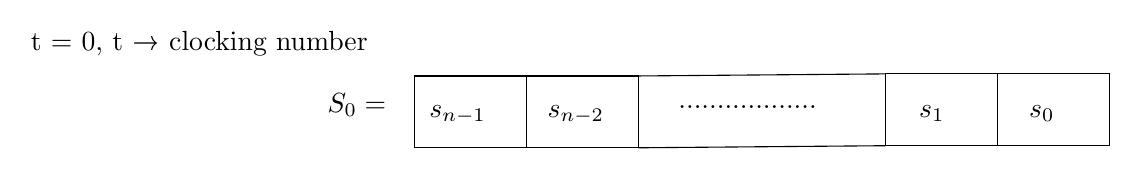
\begin{tikzpicture}[x=0.75pt,y=0.75pt,yscale=-1,xscale=1]
        \draw   (208,107) -- (262,107) -- (262,141.6) -- (208,141.6) -- cycle ; 
        \draw   (262,107) -- (316,107) -- (316,141.6) -- (262,141.6) -- cycle ;
        \draw   (435,106) -- (489,106) -- (489,140.6) -- (435,140.6) -- cycle ;
        \draw    (316,107) -- (435,106) ;
        \draw   (489,106) -- (543,106) -- (543,140.6) -- (489,140.6) -- cycle ;
        \draw    (316,141.6) -- (435,140.6) ;
        
        \draw (214,120) node [anchor=north west][inner sep=0.75pt]   [align=left] {$s_{n-1}$};
        \draw (271,120) node [anchor=north west][inner sep=0.75pt]   [align=left] {$s_{n-2}$};
        \draw (334,120) node [anchor=north west][inner sep=0.75pt]   [align=left] {..................};
        \draw (450,120) node [anchor=north west][inner sep=0.75pt]   [align=left] {$s_1$};
        \draw (503,120) node [anchor=north west][inner sep=0.75pt]   [align=left] {$s_0$};
        \draw (22,84) node [anchor=north west][inner sep=0.75pt]   [align=left] {t = 0, t → clocking number};
        \draw (165,114) node [anchor=north west][inner sep=0.75pt]   [align=left] {$S_0 = $};
    \end{tikzpicture}
\end{center}
At each clocking number, a shift by one bit takes place (either right or left, depends on the design). Here, we will take right shift for understanding.

\begin{center}
    \tikzset{every picture/.style={line width=0.75pt}} 
    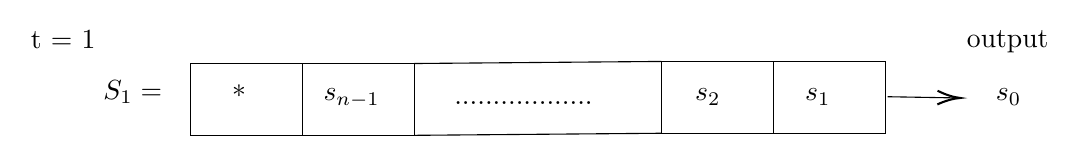
\begin{tikzpicture}[x=0.75pt,y=0.75pt,yscale=-1,xscale=1]
        \draw   (135,197) -- (189,197) -- (189,231.6) -- (135,231.6) -- cycle ;
        \draw   (189,197) -- (243,197) -- (243,231.6) -- (189,231.6) -- cycle ; 
        \draw   (362,196) -- (416,196) -- (416,230.6) -- (362,230.6) -- cycle ;
        \draw    (243,197) -- (362,196) ;
        \draw   (416,196) -- (470,196) -- (470,230.6) -- (416,230.6) -- cycle ;
        \draw    (243,231.6) -- (362,230.6) ;
        \draw    (471,213) -- (504,213.57) ;
        \draw [shift={(506,213.6)}, rotate = 180.98] [color={rgb, 255:red, 0; green, 0; blue, 0 }  ][line width=0.75]    (10.93,-3.29) .. controls (6.95,-1.4) and (3.31,-0.3) .. (0,0) .. controls (3.31,0.3) and (6.95,1.4) .. (10.93,3.29)   ;
        
        \draw (154,206) node [anchor=north west][inner sep=0.75pt]   [align=left] {*};
        \draw (198,208) node [anchor=north west][inner sep=0.75pt]   [align=left] {$s_{n-1}$};
        \draw (261,214) node [anchor=north west][inner sep=0.75pt]   [align=left] {..................};
        \draw (377,208) node [anchor=north west][inner sep=0.75pt]   [align=left] {$s_2$};
        \draw (430,208) node [anchor=north west][inner sep=0.75pt]   [align=left] {$s_1$};
        \draw (57,180) node [anchor=north west][inner sep=0.75pt]   [align=left] {t = 1};
        \draw (92,204) node [anchor=north west][inner sep=0.75pt]   [align=left] {$S_1 =$};
        \draw (508,180) node [anchor=north west][inner sep=0.75pt]   [align=left] {output};
        \draw (522,208) node [anchor=north west][inner sep=0.75pt]   [align=left] {$s_0$};
        
    \end{tikzpicture}
\end{center}

The rightmost bit $s_0$ moves out and is the output (the keystream bit). However, the leftmost bit $s_n$ becomes empty. $s_n$ is known as feedback bit and is calculated as:
\begin{center}
    $s_n = L(s_0, s_1,....., s_{n-1}) = L(S_0)$ 
\end{center}
After one more clocking, the state can be represented as:

\begin{center}
    \tikzset{every picture/.style={line width=0.75pt}} 
    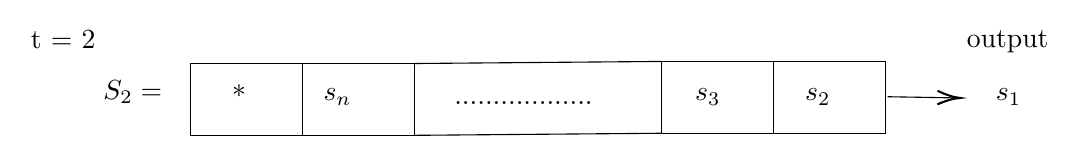
\begin{tikzpicture}[x=0.75pt,y=0.75pt,yscale=-1,xscale=1]
        \draw   (135,197) -- (189,197) -- (189,231.6) -- (135,231.6) -- cycle ;
        \draw   (189,197) -- (243,197) -- (243,231.6) -- (189,231.6) -- cycle ; 
        \draw   (362,196) -- (416,196) -- (416,230.6) -- (362,230.6) -- cycle ;
        \draw    (243,197) -- (362,196) ;
        \draw   (416,196) -- (470,196) -- (470,230.6) -- (416,230.6) -- cycle ;
        \draw    (243,231.6) -- (362,230.6) ;
        \draw    (471,213) -- (504,213.57) ;
        \draw [shift={(506,213.6)}, rotate = 180.98] [color={rgb, 255:red, 0; green, 0; blue, 0 }  ][line width=0.75]    (10.93,-3.29) .. controls (6.95,-1.4) and (3.31,-0.3) .. (0,0) .. controls (3.31,0.3) and (6.95,1.4) .. (10.93,3.29)   ;
        
        \draw (154,206) node [anchor=north west][inner sep=0.75pt]   [align=left] {*};
        \draw (198,208) node [anchor=north west][inner sep=0.75pt]   [align=left] {$s_n$};
        \draw (261,214) node [anchor=north west][inner sep=0.75pt]   [align=left] {..................};
        \draw (377,208) node [anchor=north west][inner sep=0.75pt]   [align=left] {$s_3$};
        \draw (430,208) node [anchor=north west][inner sep=0.75pt]   [align=left] {$s_2$};
        \draw (57,180) node [anchor=north west][inner sep=0.75pt]   [align=left] {t = 2};
        \draw (92,204) node [anchor=north west][inner sep=0.75pt]   [align=left] {$S_2 =$};
        \draw (508,180) node [anchor=north west][inner sep=0.75pt]   [align=left] {output};
        \draw (522,208) node [anchor=north west][inner sep=0.75pt]   [align=left] {$s_1$};
        
    \end{tikzpicture}
\end{center}
Again, the feedback bit $S_{n+1} = L(S_1)$. We will look at the function L in some time. The LFSR with right shift operation can be represented with the following circuit.
\begin{center}
    \tikzset{every picture/.style={line width=0.75pt}} 
    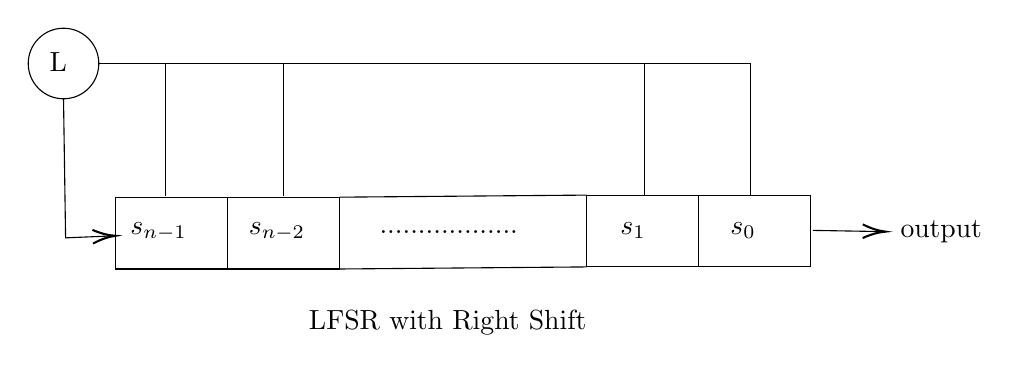
\begin{tikzpicture}[x=0.75pt,y=0.75pt,yscale=-1,xscale=1]
        \draw   (138,147) -- (192,147) -- (192,181.6) -- (138,181.6) -- cycle ;
        \draw   (192,147) -- (246,147) -- (246,181.6) -- (192,181.6) -- cycle ;
        \draw   (365,146) -- (419,146) -- (419,180.6) -- (365,180.6) -- cycle ; 
        \draw    (246,147) -- (365,146) ;
        \draw   (419,146) -- (473,146) -- (473,180.6) -- (419,180.6) -- cycle ;
        \draw    (246,181.6) -- (365,180.6) ; 
        \draw    (474,163) -- (507,163.57) ;
        \draw [shift={(509,163.6)}, rotate = 180.98] [color={rgb, 255:red, 0; green, 0; blue, 0 }  ][line width=0.75]    (10.93,-3.29) .. controls (6.95,-1.4) and (3.31,-0.3) .. (0,0) .. controls (3.31,0.3) and (6.95,1.4) .. (10.93,3.29)   ;
        \draw    (130,82.6) -- (444,82.6) -- (444,146) ;
        \draw   (96,82.6) .. controls (96,73.21) and (103.61,65.6) .. (113,65.6) .. controls (122.39,65.6) and (130,73.21) .. (130,82.6) .. controls (130,91.99) and (122.39,99.6) .. (113,99.6) .. controls (103.61,99.6) and (96,91.99) .. (96,82.6) -- cycle ;
        \draw    (113,99.6) -- (114,166.6) -- (136,165.68) ;
        \draw [shift={(138,165.6)}, rotate = 177.61] [color={rgb, 255:red, 0; green, 0; blue, 0 }  ][line width=0.75]    (10.93,-3.29) .. controls (6.95,-1.4) and (3.31,-0.3) .. (0,0) .. controls (3.31,0.3) and (6.95,1.4) .. (10.93,3.29)   ;
        \draw    (162,82.6) -- (162,146.6) ;
        \draw    (219,82.6) -- (219,146.6) ;
        \draw    (393,82.6) -- (393,146.6) ;
        
        \draw (144,158) node [anchor=north west][inner sep=0.75pt]   [align=left] {$s_{n-1}$};
        \draw (201,158) node [anchor=north west][inner sep=0.75pt]   [align=left] {$s_{n-2}$};
        \draw (264,162) node [anchor=north west][inner sep=0.75pt]   [align=left] {..................};
        \draw (380,158) node [anchor=north west][inner sep=0.75pt]   [align=left] {$s_1$};
        \draw (433,158) node [anchor=north west][inner sep=0.75pt]   [align=left] {$s_0$};
        \draw (515,157) node [anchor=north west][inner sep=0.75pt]   [align=left] {output};
        \draw (105,76) node [anchor=north west][inner sep=0.75pt]   [align=left] {L};
        \draw (230,200) node [anchor=north west][inner sep=0.75pt]   [align=left] {LFSR with Right Shift};
    \end{tikzpicture}
\end{center}

The function L is a linear function on the bits of the previous state.
\begin{center}
    $L: \{0,1\}^n \rightarrow \{0,1\}$\\
    $L(s_0, s_1,....., s_{n-1}) = s_n$
\end{center}
A linear function can be represented as:
\begin{center}
    $L_a = a_0\cdot s_0 \oplus a_1 \cdot s_1 \oplus ..... \oplus a_{n-1} \cdot s_{n-1}$ where $a_i \in \{0, 1\}$
\end{center}

Suppose, an arbitrary function L be defined as:
\begin{center}
    $L = a_0\cdot s_0 \oplus a_1 \cdot s_1 \oplus ..... \oplus a_{n-1} \cdot s_{n-1} \oplus a_n$ where $a_i \in \{0, 1\}$
\end{center}
In this function, if $a_n = 0$ then $L = L_a$, a linear function. Otherwise, if $a_n = 1$ the $L \neq L_a$. In fact, such a function is known as Affine function.

A function can be proved to be linear using the following property.
\begin{center}
    $L(X) \oplus L(Y) = L(X \oplus Y)$\\
    $\implies L(X) \oplus L(Y) \oplus L(X \oplus Y) = 0$
\end{center}
\textbf{Example:} Find if the following functions are linear or not. Solve it considering 2-bit inputs.
\begin{enumerate}
    \item $L_1(x, y) = x \oplus y$
    \item $L_2(x, y) = 1 \oplus x \oplus y$

\end{enumerate}
\textbf{Solution:} 
\begin{enumerate}
    \item Let's compute $L_1(x) \oplus L_1(y) \oplus L_1(x \oplus y)$
    \begin{center}
        $L_1(x) \oplus L_1(y) \oplus L_1(x \oplus y) = (x_1 \oplus x_2) \oplus (y_1 \oplus y_2) \oplus ((x_1 \oplus y_1) \oplus (x_2 \oplus y_2))$\\
        \vspace{1mm}
        $L_1(x) \oplus L_1(y) \oplus L_1(x \oplus y) = 0$
    \end{center}
    Therefore, $L_1$ is a linear function.
    \item $L_2(x) \oplus L_2(y) \oplus L_2(x \oplus y) = (1 \oplus x_1 \oplus x_2) \oplus (1 \oplus y_1 \oplus y_2) \oplus (1 \oplus (x_1 \oplus y_1) \oplus (x_2 \oplus y_2))$
    \begin{center}
        $L_2(x) \oplus L_2(y) \oplus L_2(x \oplus y) = 1 $
    \end{center}
    Therefore, $L_2$ is not a linear function.
\end{enumerate}

LFSR has a linear function, whose output depends on previous state, therefore it provides feedback. There is shift operation on the bits stored in register. Hence, the name is Linear Feedback Shift Register. \\
Now, let us see an example of a 3-bit LFSR.

\begin{center}
    \tikzset{every picture/.style={line width=0.75pt}}
    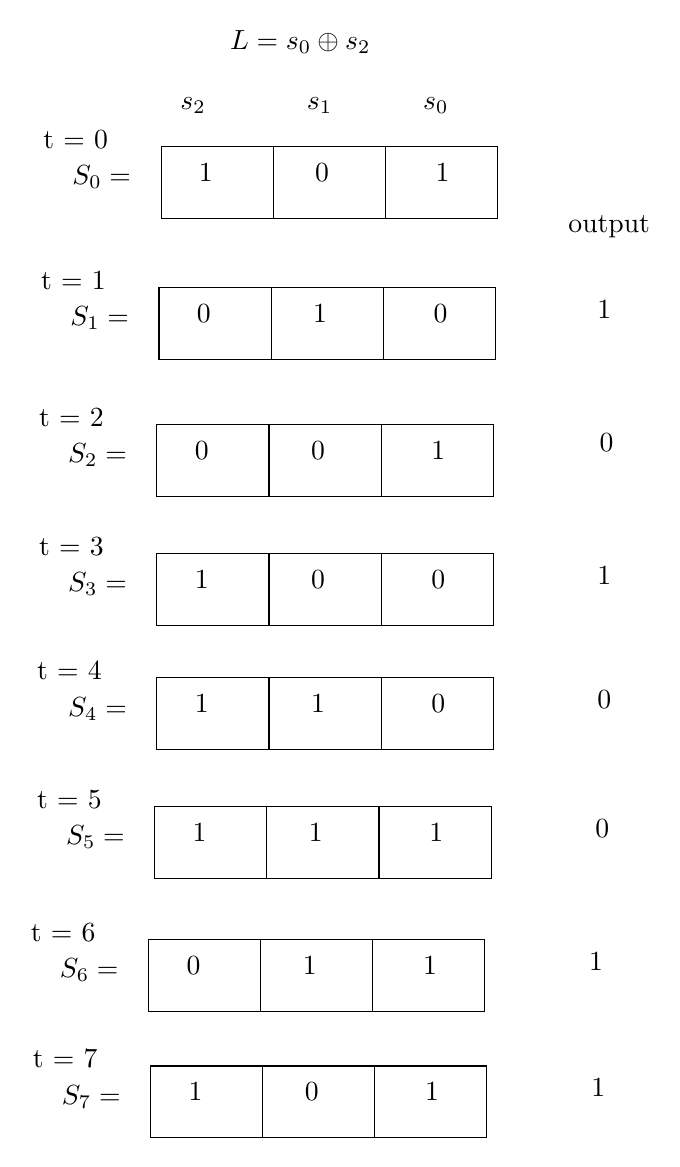
\begin{tikzpicture}[x=0.75pt,y=0.75pt,yscale=-1,xscale=1]
        
        \draw   (230,277) -- (284,277) -- (284,311.6) -- (230,311.6) -- cycle ;
        \draw   (284,277) -- (338,277) -- (338,311.6) -- (284,311.6) -- cycle ;
        \draw   (338,277) -- (392,277) -- (392,311.6) -- (338,311.6) -- cycle ;
        \draw   (229,345) -- (283,345) -- (283,379.6) -- (229,379.6) -- cycle ;
        \draw   (283,345) -- (337,345) -- (337,379.6) -- (283,379.6) -- cycle ;
        \draw   (337,345) -- (391,345) -- (391,379.6) -- (337,379.6) -- cycle ;
        \draw   (228,411) -- (282,411) -- (282,445.6) -- (228,445.6) -- cycle ;
        \draw   (282,411) -- (336,411) -- (336,445.6) -- (282,445.6) -- cycle ;
        \draw   (336,411) -- (390,411) -- (390,445.6) -- (336,445.6) -- cycle ;
        \draw   (228,473) -- (282,473) -- (282,507.6) -- (228,507.6) -- cycle ;
        \draw   (282,473) -- (336,473) -- (336,507.6) -- (282,507.6) -- cycle ;
        \draw   (336,473) -- (390,473) -- (390,507.6) -- (336,507.6) -- cycle ;
        \draw   (228,533) -- (282,533) -- (282,567.6) -- (228,567.6) -- cycle ;
        \draw   (282,533) -- (336,533) -- (336,567.6) -- (282,567.6) -- cycle ;
        \draw   (336,533) -- (390,533) -- (390,567.6) -- (336,567.6) -- cycle ;
        \draw   (227,595) -- (281,595) -- (281,629.6) -- (227,629.6) -- cycle ;
        \draw   (281,595) -- (335,595) -- (335,629.6) -- (281,629.6) -- cycle ;
        \draw   (335,595) -- (389,595) -- (389,629.6) -- (335,629.6) -- cycle ;
        \draw   (224,659) -- (278,659) -- (278,693.6) -- (224,693.6) -- cycle ;
        \draw   (278,659) -- (332,659) -- (332,693.6) -- (278,693.6) -- cycle ;
        \draw   (332,659) -- (386,659) -- (386,693.6) -- (332,693.6) -- cycle ;
        \draw   (225,720) -- (279,720) -- (279,754.6) -- (225,754.6) -- cycle ;
        \draw   (279,720) -- (333,720) -- (333,754.6) -- (279,754.6) -- cycle ;
        \draw   (333,720) -- (387,720) -- (387,754.6) -- (333,754.6) -- cycle ;
        
        \draw (303,284) node [anchor=north west][inner sep=0.75pt]   [align=left] {0};
        \draw (262,220) node [anchor=north west][inner sep=0.75pt]   [align=left] {$L = s_0 \oplus s_2$};
        \draw (238,252) node [anchor=north west][inner sep=0.75pt]   [align=left] {$s_2$};
        \draw (299,252) node [anchor=north west][inner sep=0.75pt]   [align=left] {$s_1$};
        \draw (355,252) node [anchor=north west][inner sep=0.75pt]   [align=left] {$s_0$};
        \draw (172,268) node [anchor=north west][inner sep=0.75pt]   [align=left] {t = 0};
        \draw (186,285) node [anchor=north west][inner sep=0.75pt]   [align=left] {$S_0 = $};
        \draw (425,309) node [anchor=north west][inner sep=0.75pt]   [align=left] {output};
        \draw (247,284) node [anchor=north west][inner sep=0.75pt]   [align=left] {1};
        \draw (361,284) node [anchor=north west][inner sep=0.75pt]   [align=left] {1};
        \draw (302,352) node [anchor=north west][inner sep=0.75pt]   [align=left] {1};
        \draw (171,336) node [anchor=north west][inner sep=0.75pt]   [align=left] {t = 1};
        \draw (185,353) node [anchor=north west][inner sep=0.75pt]   [align=left] {$S_1 = $};
        \draw (246,352) node [anchor=north west][inner sep=0.75pt]   [align=left] {0};
        \draw (360,352) node [anchor=north west][inner sep=0.75pt]   [align=left] {0};
        \draw (301,418) node [anchor=north west][inner sep=0.75pt]   [align=left] {0};
        \draw (170,402) node [anchor=north west][inner sep=0.75pt]   [align=left] {t = 2};
        \draw (184,419) node [anchor=north west][inner sep=0.75pt]   [align=left] {$S_2 = $};
        \draw (245,418) node [anchor=north west][inner sep=0.75pt]   [align=left] {0};
        \draw (359,418) node [anchor=north west][inner sep=0.75pt]   [align=left] {1};
        \draw (301,480) node [anchor=north west][inner sep=0.75pt]   [align=left] {0};
        \draw (170,464) node [anchor=north west][inner sep=0.75pt]   [align=left] {t = 3};
        \draw (184,481) node [anchor=north west][inner sep=0.75pt]   [align=left] {$S_3 = $};
        \draw (245,480) node [anchor=north west][inner sep=0.75pt]   [align=left] {1};
        \draw (359,480) node [anchor=north west][inner sep=0.75pt]   [align=left] {0};
        \draw (439,350) node [anchor=north west][inner sep=0.75pt]   [align=left] {1};
        \draw (440,414) node [anchor=north west][inner sep=0.75pt]   [align=left] {0};
        \draw (439,478) node [anchor=north west][inner sep=0.75pt]   [align=left] {1};
        \draw (301,540) node [anchor=north west][inner sep=0.75pt]   [align=left] {1};
        \draw (169,524) node [anchor=north west][inner sep=0.75pt]   [align=left] {t = 4};
        \draw (184,541) node [anchor=north west][inner sep=0.75pt]   [align=left] {$S_4 = $};
        \draw (245,540) node [anchor=north west][inner sep=0.75pt]   [align=left] {1};
        \draw (359,540) node [anchor=north west][inner sep=0.75pt]   [align=left] {0};
        \draw (439,538) node [anchor=north west][inner sep=0.75pt]   [align=left] {0};
        \draw (300,602) node [anchor=north west][inner sep=0.75pt]   [align=left] {1};
        \draw (169,586) node [anchor=north west][inner sep=0.75pt]   [align=left] {t = 5};
        \draw (183,603) node [anchor=north west][inner sep=0.75pt]   [align=left] {$S_5 = $};
        \draw (244,602) node [anchor=north west][inner sep=0.75pt]   [align=left] {1};
        \draw (358,602) node [anchor=north west][inner sep=0.75pt]   [align=left] {1};
        \draw (438,600) node [anchor=north west][inner sep=0.75pt]   [align=left] {0};
        \draw (297,666) node [anchor=north west][inner sep=0.75pt]   [align=left] {1};
        \draw (166,650) node [anchor=north west][inner sep=0.75pt]   [align=left] {t = 6};
        \draw (180,667) node [anchor=north west][inner sep=0.75pt]   [align=left] {$S_6 = $};
        \draw (241,666) node [anchor=north west][inner sep=0.75pt]   [align=left] {0};
        \draw (355,666) node [anchor=north west][inner sep=0.75pt]   [align=left] {1};
        \draw (435,664) node [anchor=north west][inner sep=0.75pt]   [align=left] {1};
        \draw (298,727) node [anchor=north west][inner sep=0.75pt]   [align=left] {0};
        \draw (167,711) node [anchor=north west][inner sep=0.75pt]   [align=left] {t = 7};
        \draw (181,728) node [anchor=north west][inner sep=0.75pt]   [align=left] {$S_7 = $};
        \draw (242,727) node [anchor=north west][inner sep=0.75pt]   [align=left] {1};
        \draw (356,727) node [anchor=north west][inner sep=0.75pt]   [align=left] {1};
        \draw (436,725) node [anchor=north west][inner sep=0.75pt]   [align=left] {1};        
    \end{tikzpicture}
\end{center}

The L function for this LFSR is $L = s_0 \oplus s_2$.\\
In any LFSR, if you have reached the initial state again, the the output bits will be repeated. In the above example it can be seen that from start state t = 0 to the state t = 7, all the non-zero states are obtained.\\
The output bits in the above example are repeated after $t = 2^3 - 1$ states because at t = 7, the initial state is reached. Hence, maximum output length that can be achieved in this LFSR without repetition is 7.
Hence, using LFSR, only $2^n - 1$ maximum number of non-zero states can be generated.\\
Also, if we take the 0 state i.e. all bits in the register are 0, it will remain in the zero state forever. Hence, in any LFSR, if input state is 0, then it will remain zero. Hence, LFSR has a fixed point (0-state).\\

Let us look at another example of a 3-bit LFSR with a different L function. This time the L function is $L = s_0$.

\begin{center}   
    \tikzset{every picture/.style={line width=0.75pt}}
    \begin{tikzpicture}[x=0.75pt,y=0.75pt,yscale=-1,xscale=1]
        \draw   (230,277) -- (284,277) -- (284,311.6) -- (230,311.6) -- cycle ;
        \draw   (284,277) -- (338,277) -- (338,311.6) -- (284,311.6) -- cycle ; 
        \draw   (338,277) -- (392,277) -- (392,311.6) -- (338,311.6) -- cycle ; 
        \draw   (229,345) -- (283,345) -- (283,379.6) -- (229,379.6) -- cycle ;
        \draw   (283,345) -- (337,345) -- (337,379.6) -- (283,379.6) -- cycle ;
        \draw   (337,345) -- (391,345) -- (391,379.6) -- (337,379.6) -- cycle ;
        \draw   (228,411) -- (282,411) -- (282,445.6) -- (228,445.6) -- cycle ;
        \draw   (282,411) -- (336,411) -- (336,445.6) -- (282,445.6) -- cycle ;
        \draw   (336,411) -- (390,411) -- (390,445.6) -- (336,445.6) -- cycle ;
        \draw   (228,473) -- (282,473) -- (282,507.6) -- (228,507.6) -- cycle ;
        \draw   (282,473) -- (336,473) -- (336,507.6) -- (282,507.6) -- cycle ;
        \draw   (336,473) -- (390,473) -- (390,507.6) -- (336,507.6) -- cycle ;
        
        
        \draw (303,284) node [anchor=north west][inner sep=0.75pt]   [align=left] {0};
        \draw (290,220) node [anchor=north west][inner sep=0.75pt]   [align=left] {$L = s0$};
        \draw (238,252) node [anchor=north west][inner sep=0.75pt]   [align=left] {$s_2$};
        \draw (299,252) node [anchor=north west][inner sep=0.75pt]   [align=left] {$s_1$};
        \draw (355,252) node [anchor=north west][inner sep=0.75pt]   [align=left] {$s_0$};
        \draw (172,268) node [anchor=north west][inner sep=0.75pt]   [align=left] {t = 0};
        \draw (186,285) node [anchor=north west][inner sep=0.75pt]   [align=left] {$S_0 = $};
        \draw (425,309) node [anchor=north west][inner sep=0.75pt]   [align=left] {output};
        \draw (247,284) node [anchor=north west][inner sep=0.75pt]   [align=left] {1};
        \draw (361,284) node [anchor=north west][inner sep=0.75pt]   [align=left] {1};
        \draw (302,352) node [anchor=north west][inner sep=0.75pt]   [align=left] {1};
        \draw (171,336) node [anchor=north west][inner sep=0.75pt]   [align=left] {t = 1};
        \draw (185,353) node [anchor=north west][inner sep=0.75pt]   [align=left] {$S_1 = $};
        \draw (246,352) node [anchor=north west][inner sep=0.75pt]   [align=left] {1};
        \draw (360,352) node [anchor=north west][inner sep=0.75pt]   [align=left] {0};
        \draw (301,418) node [anchor=north west][inner sep=0.75pt]   [align=left] {1};
        \draw (170,402) node [anchor=north west][inner sep=0.75pt]   [align=left] {t = 2};
        \draw (184,419) node [anchor=north west][inner sep=0.75pt]   [align=left] {$S_2 = $};
        \draw (245,418) node [anchor=north west][inner sep=0.75pt]   [align=left] {0};
        \draw (359,418) node [anchor=north west][inner sep=0.75pt]   [align=left] {1};
        \draw (301,480) node [anchor=north west][inner sep=0.75pt]   [align=left] {0};
        \draw (170,464) node [anchor=north west][inner sep=0.75pt]   [align=left] {t = 3};
        \draw (184,481) node [anchor=north west][inner sep=0.75pt]   [align=left] {$S_3 = $};
        \draw (245,480) node [anchor=north west][inner sep=0.75pt]   [align=left] {1};
        \draw (359,480) node [anchor=north west][inner sep=0.75pt]   [align=left] {1};
        \draw (439,350) node [anchor=north west][inner sep=0.75pt]   [align=left] {1};
        \draw (440,414) node [anchor=north west][inner sep=0.75pt]   [align=left] {0};
        \draw (439,478) node [anchor=north west][inner sep=0.75pt]   [align=left] {1};        
    \end{tikzpicture}
\end{center}
Here, we can see the initial state is reached again only at t = 3. For LFSR, the linear functionis very important in deciding the period after which the bits will repeat.

\subsubsection*{Period of an LFSR} 
Consider $S_0$ to be a non-zero state. $S_0$ is repeated after $m$ clocking of LFSR, then $m$ will be the period of LFSR. An LFSR with n-bits can have a maximum period of $2^n - 1$.\\


If there is an LFSR where different non-zero states are repeating at certain different number of clocking. Let us say $x_1$ number of states repeat after $P_1$ clocking, $x_2$ number of states repeat after $P_2$ clocking and so on $x_n$ number of states repeat after $P_N$ clocking. Here, every non-zero state is present in at least and only one $x_i$. Therefore, if we take any non-zero state, then it will repeat after certain number of clocking which will belong to the set $\{P_1, P_2,...., P_N\}$. Therefore, the period of LFSR will be:
\begin{center}
    Period of LFSR = $LCM(P_1, P_2,...., P_N)$
\end{center}
Consider an n-bit LFSR,
\begin{center}
    \tikzset{every picture/.style={line width=0.75pt}} 
    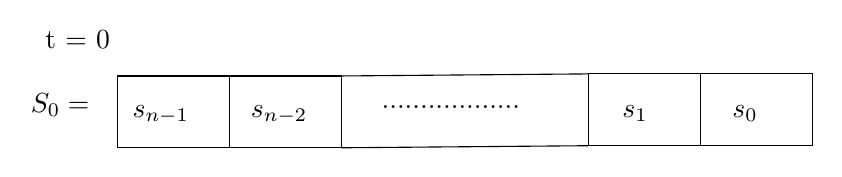
\begin{tikzpicture}[x=0.75pt,y=0.75pt,yscale=-1,xscale=1]
        \draw   (208,107) -- (262,107) -- (262,141.6) -- (208,141.6) -- cycle ; 
        \draw   (262,107) -- (316,107) -- (316,141.6) -- (262,141.6) -- cycle ;
        \draw   (435,106) -- (489,106) -- (489,140.6) -- (435,140.6) -- cycle ;
        \draw    (316,107) -- (435,106) ;
        \draw   (489,106) -- (543,106) -- (543,140.6) -- (489,140.6) -- cycle ;
        \draw    (316,141.6) -- (435,140.6) ;
        
        \draw (214,120) node [anchor=north west][inner sep=0.75pt]   [align=left] {$s_{n-1}$};
        \draw (271,120) node [anchor=north west][inner sep=0.75pt]   [align=left] {$s_{n-2}$};
        \draw (334,120) node [anchor=north west][inner sep=0.75pt]   [align=left] {..................};
        \draw (450,120) node [anchor=north west][inner sep=0.75pt]   [align=left] {$s_1$};
        \draw (503,120) node [anchor=north west][inner sep=0.75pt]   [align=left] {$s_0$};
        \draw (172,84) node [anchor=north west][inner sep=0.75pt]   [align=left] {t = 0};
        \draw (165,114) node [anchor=north west][inner sep=0.75pt]   [align=left] {$S_0 = $};
    \end{tikzpicture}
\end{center}
We know that after clocking, $s_n$ will be,
\begin{center}
    $s_n = L(s_0,s_1,...., s_{n-1})$\\
    $s_n = c_1\cdot s_{n-1} \oplus c_2 \cdot s_{n-2} \oplus ..... \oplus c_n \cdot s_0$ where $c_i \in \{0, 1\}$
\end{center}
This is known as Algebraic Normal Form of writing $s_n$. Therefore, we can see that to implement LFSR in hardware, we only need AND and XOR gates. The circuit for LFSR is given below. The value of $s_i$ will be xored or not depends on the value of $c_{n-i}$.

\begin{center}
    \tikzset{every picture/.style={line width=0.75pt}} 
    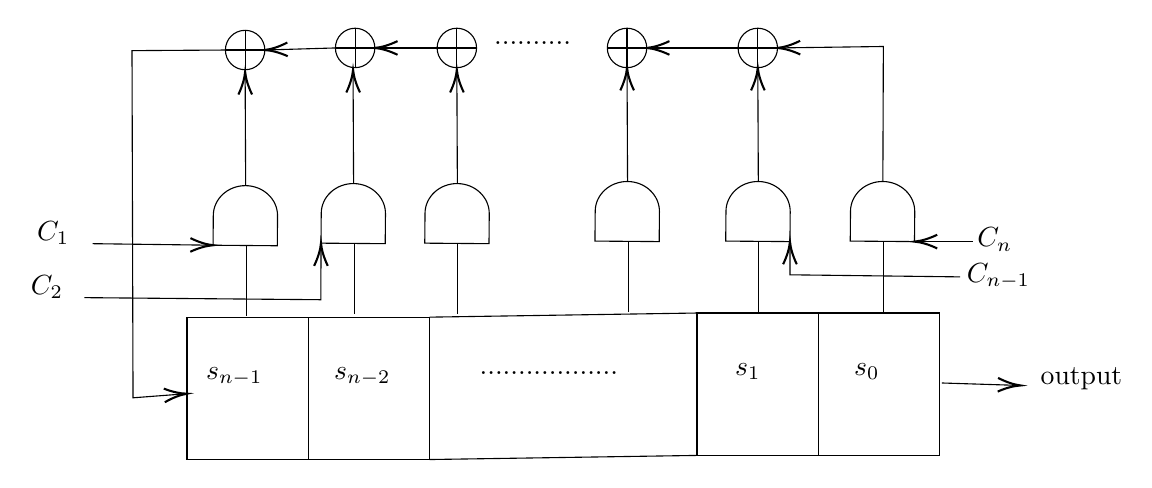
\begin{tikzpicture}[x=0.75pt,y=0.75pt,yscale=-1,xscale=1]
        \draw   (110.47,177.2) -- (168.93,177.2) -- (168.93,245.8) -- (110.47,245.8) -- cycle ;
        \draw   (168.93,177.2) -- (227.39,177.2) -- (227.39,245.8) -- (168.93,245.8) -- cycle ;
        \draw   (356.22,175.21) -- (414.68,175.21) -- (414.68,243.82) -- (356.22,243.82) -- cycle ; 
        \draw    (227.39,177.2) -- (356.22,175.21) ;
        \draw   (414.68,175.21) -- (473.14,175.21) -- (473.14,243.82) -- (414.68,243.82) -- cycle ;
        \draw    (227.39,245.8) -- (356.22,243.82) ;
        \draw    (474.22,208.92) -- (510.11,210.05) ;
        \draw [shift={(512.11,210.11)}, rotate = 181.8] [color={rgb, 255:red, 0; green, 0; blue, 0 }  ][line width=0.75]    (10.93,-3.29) .. controls (6.95,-1.4) and (3.31,-0.3) .. (0,0) .. controls (3.31,0.3) and (6.95,1.4) .. (10.93,3.29)   ;
        \draw    (129,48.5) -- (84,48.8) -- (84.49,216.06) -- (108.47,214.23) ;
        \draw [shift={(110.47,214.08)}, rotate = 175.64] [color={rgb, 255:red, 0; green, 0; blue, 0 }  ][line width=0.75]    (10.93,-3.29) .. controls (6.95,-1.4) and (3.31,-0.3) .. (0,0) .. controls (3.31,0.3) and (6.95,1.4) .. (10.93,3.29)   ;
        \draw   (370.05,140.55) -- (370.17,126.13) .. controls (370.24,118.17) and (377.22,111.77) .. (385.76,111.84) .. controls (394.31,111.91) and (401.18,118.42) .. (401.12,126.38) -- (401,140.8) -- cycle ;
        \draw    (386,140.8) -- (386,174.8) ; 
        \draw   (129,48.5) .. controls (129,43.25) and (133.25,39) .. (138.5,39) .. controls (143.75,39) and (148,43.25) .. (148,48.5) .. controls (148,53.75) and (143.75,58) .. (138.5,58) .. controls (133.25,58) and (129,53.75) .. (129,48.5) -- cycle ; \draw   (129,48.5) -- (148,48.5) ; \draw   (138.5,39) -- (138.5,58) ;
        \draw   (182,47.5) .. controls (182,42.25) and (186.25,38) .. (191.5,38) .. controls (196.75,38) and (201,42.25) .. (201,47.5) .. controls (201,52.75) and (196.75,57) .. (191.5,57) .. controls (186.25,57) and (182,52.75) .. (182,47.5) -- cycle ; \draw   (182,47.5) -- (201,47.5) ; \draw   (191.5,38) -- (191.5,57) ;
        \draw   (231,47.5) .. controls (231,42.25) and (235.25,38) .. (240.5,38) .. controls (245.75,38) and (250,42.25) .. (250,47.5) .. controls (250,52.75) and (245.75,57) .. (240.5,57) .. controls (235.25,57) and (231,52.75) .. (231,47.5) -- cycle ; \draw   (231,47.5) -- (250,47.5) ; \draw   (240.5,38) -- (240.5,57) ;
        \draw   (313,47.5) .. controls (313,42.25) and (317.25,38) .. (322.5,38) .. controls (327.75,38) and (332,42.25) .. (332,47.5) .. controls (332,52.75) and (327.75,57) .. (322.5,57) .. controls (317.25,57) and (313,52.75) .. (313,47.5) -- cycle ; \draw   (313,47.5) -- (332,47.5) ; \draw   (322.5,38) -- (322.5,57) ;
        \draw   (376,47.5) .. controls (376,42.25) and (380.25,38) .. (385.5,38) .. controls (390.75,38) and (395,42.25) .. (395,47.5) .. controls (395,52.75) and (390.75,57) .. (385.5,57) .. controls (380.25,57) and (376,52.75) .. (376,47.5) -- cycle ; \draw   (376,47.5) -- (395,47.5) ; \draw   (385.5,38) -- (385.5,57) ;
        \draw    (376,47.5) -- (334,47.5) ;
        \draw [shift={(332,47.5)}, rotate = 360] [color={rgb, 255:red, 0; green, 0; blue, 0 }  ][line width=0.75]    (10.93,-3.29) .. controls (6.95,-1.4) and (3.31,-0.3) .. (0,0) .. controls (3.31,0.3) and (6.95,1.4) .. (10.93,3.29)   ;
        \draw    (231,47.5) -- (203,47.5) ;
        \draw [shift={(201,47.5)}, rotate = 360] [color={rgb, 255:red, 0; green, 0; blue, 0 }  ][line width=0.75]    (10.93,-3.29) .. controls (6.95,-1.4) and (3.31,-0.3) .. (0,0) .. controls (3.31,0.3) and (6.95,1.4) .. (10.93,3.29)   ;
        \draw    (182,47.5) -- (150,48.44) ;
        \draw [shift={(148,48.5)}, rotate = 358.32] [color={rgb, 255:red, 0; green, 0; blue, 0 }  ][line width=0.75]    (10.93,-3.29) .. controls (6.95,-1.4) and (3.31,-0.3) .. (0,0) .. controls (3.31,0.3) and (6.95,1.4) .. (10.93,3.29)   ;
        \draw    (385.76,111.84) -- (385.51,59) ;
        \draw [shift={(385.5,57)}, rotate = 89.73] [color={rgb, 255:red, 0; green, 0; blue, 0 }  ][line width=0.75]    (10.93,-3.29) .. controls (6.95,-1.4) and (3.31,-0.3) .. (0,0) .. controls (3.31,0.3) and (6.95,1.4) .. (10.93,3.29)   ;
        \draw   (307.05,140.55) -- (307.17,126.13) .. controls (307.24,118.17) and (314.22,111.77) .. (322.76,111.84) .. controls (331.31,111.91) and (338.18,118.42) .. (338.12,126.38) -- (338,140.8) -- cycle ;
        \draw    (323,140.8) -- (323,174.8) ;
        \draw    (322.76,111.84) -- (322.51,59) ;
        \draw [shift={(322.5,57)}, rotate = 89.73] [color={rgb, 255:red, 0; green, 0; blue, 0 }  ][line width=0.75]    (10.93,-3.29) .. controls (6.95,-1.4) and (3.31,-0.3) .. (0,0) .. controls (3.31,0.3) and (6.95,1.4) .. (10.93,3.29)   ;
        \draw   (225.05,141.55) -- (225.17,127.13) .. controls (225.24,119.17) and (232.22,112.77) .. (240.76,112.84) .. controls (249.31,112.91) and (256.18,119.42) .. (256.12,127.38) -- (256,141.8) -- cycle ;
        \draw    (241,141.8) -- (241,175.8) ; 
        \draw    (240.76,112.84) -- (240.51,60) ;
        \draw [shift={(240.5,58)}, rotate = 89.73] [color={rgb, 255:red, 0; green, 0; blue, 0 }  ][line width=0.75]    (10.93,-3.29) .. controls (6.95,-1.4) and (3.31,-0.3) .. (0,0) .. controls (3.31,0.3) and (6.95,1.4) .. (10.93,3.29)   ;
        \draw   (175.05,141.55) -- (175.17,127.13) .. controls (175.24,119.17) and (182.22,112.77) .. (190.76,112.84) .. controls (199.31,112.91) and (206.18,119.42) .. (206.12,127.38) -- (206,141.8) -- cycle ;
        \draw    (191,141.8) -- (191,175.8) ; 
        \draw    (190.76,112.84) -- (190.51,60) ;
        \draw [shift={(190.5,58)}, rotate = 89.73] [color={rgb, 255:red, 0; green, 0; blue, 0 }  ][line width=0.75]    (10.93,-3.29) .. controls (6.95,-1.4) and (3.31,-0.3) .. (0,0) .. controls (3.31,0.3) and (6.95,1.4) .. (10.93,3.29)   ; 
        \draw   (123.05,142.55) -- (123.17,128.13) .. controls (123.24,120.17) and (130.22,113.77) .. (138.76,113.84) .. controls (147.31,113.91) and (154.18,120.42) .. (154.12,128.38) -- (154,142.8) -- cycle ;
        \draw    (139,142.8) -- (139,176.8) ;
        \draw    (138.76,113.84) -- (138.51,61) ;
        \draw [shift={(138.5,59)}, rotate = 89.73] [color={rgb, 255:red, 0; green, 0; blue, 0 }  ][line width=0.75]    (10.93,-3.29) .. controls (6.95,-1.4) and (3.31,-0.3) .. (0,0) .. controls (3.31,0.3) and (6.95,1.4) .. (10.93,3.29)   ;
        \draw   (430.05,140.55) -- (430.17,126.13) .. controls (430.24,118.17) and (437.22,111.77) .. (445.76,111.84) .. controls (454.31,111.91) and (461.18,118.42) .. (461.12,126.38) -- (461,140.8) -- cycle ;
        \draw    (446,140.8) -- (446,174.8) ;
        \draw    (445.76,111.84) -- (446,46.8) -- (397,47.47) ;
        \draw [shift={(395,47.5)}, rotate = 359.21] [color={rgb, 255:red, 0; green, 0; blue, 0 }  ][line width=0.75]    (10.93,-3.29) .. controls (6.95,-1.4) and (3.31,-0.3) .. (0,0) .. controls (3.31,0.3) and (6.95,1.4) .. (10.93,3.29)   ;
        \draw    (489,140.8) -- (463,140.8) ;
        \draw [shift={(461,140.8)}, rotate = 360] [color={rgb, 255:red, 0; green, 0; blue, 0 }  ][line width=0.75]    (10.93,-3.29) .. controls (6.95,-1.4) and (3.31,-0.3) .. (0,0) .. controls (3.31,0.3) and (6.95,1.4) .. (10.93,3.29)   ;
        \draw    (483,157.8) -- (401,156.8) -- (401,142.8) ;
        \draw [shift={(401,140.8)}, rotate = 90] [color={rgb, 255:red, 0; green, 0; blue, 0 }  ][line width=0.75]    (10.93,-3.29) .. controls (6.95,-1.4) and (3.31,-0.3) .. (0,0) .. controls (3.31,0.3) and (6.95,1.4) .. (10.93,3.29)   ;
        \draw    (61,167.8) -- (175,168.8) -- (175.05,143.55) ;
        \draw [shift={(175.05,141.55)}, rotate = 90.11] [color={rgb, 255:red, 0; green, 0; blue, 0 }  ][line width=0.75]    (10.93,-3.29) .. controls (6.95,-1.4) and (3.31,-0.3) .. (0,0) .. controls (3.31,0.3) and (6.95,1.4) .. (10.93,3.29)   ;
        \draw    (65,141.8) -- (121.05,142.52) ;
        \draw [shift={(123.05,142.55)}, rotate = 180.74] [color={rgb, 255:red, 0; green, 0; blue, 0 }  ][line width=0.75]    (10.93,-3.29) .. controls (6.95,-1.4) and (3.31,-0.3) .. (0,0) .. controls (3.31,0.3) and (6.95,1.4) .. (10.93,3.29)   ;
        
        \draw (118.41,200.39) node [anchor=north west][inner sep=0.75pt]   [align=left] {$s_{n-1}$};
        \draw (180.12,200.39) node [anchor=north west][inner sep=0.75pt]   [align=left] {$s_{n-2}$};
        \draw (250.22,202.38) node [anchor=north west][inner sep=0.75pt]   [align=left] {..................};
        \draw (373.32,198.41) node [anchor=north west][inner sep=0.75pt]   [align=left] {$s_1$};
        \draw (430.7,198.41) node [anchor=north west][inner sep=0.75pt]   [align=left] {$s_0$};
        \draw (520.55,200.39) node [anchor=north west][inner sep=0.75pt]   [align=left] {output};
        \draw (257.22,43.38) node [anchor=north west][inner sep=0.75pt]   [align=left] {..........};
        \draw (490,133) node [anchor=north west][inner sep=0.75pt]   [align=left] {$C_n$};
        \draw (485,150) node [anchor=north west][inner sep=0.75pt]   [align=left] {$C_{n-1}$};
        \draw (34,156) node [anchor=north west][inner sep=0.75pt]   [align=left] {$C_2$};
        \draw (37,130) node [anchor=north west][inner sep=0.75pt]   [align=left] {$C_1$};        
    \end{tikzpicture}
\end{center}



Corresponding to every LFSR, we have a Linear Feedback Function (L). Corresponding to LFF, we can construct a polynomial $f(x)$.
\begin{center}
    $L = c_1\cdot s_{n-1} \oplus c_2 \cdot s_{n-2} \oplus ..... \oplus c_n \cdot s_0$\\
    $f(x) = 1 + c_1 \cdot x + c_2 \cdot x^2 + ..... + c_n \cdot x^n$
\end{center}
The polynomial $f(x)$ is known as connection polynomial of LFSR. If anyone of the linear feedback function or the connection poylnomial is known, the other can be easily constructed. Since, $c_i \in \{0, 1\}$ for $1 \leq i \leq n$, therefore, $f(x) \in F_2[x]$. Therefore, 
\begin{center}
    n-bit LFSR $\iff$ Linear Feedback Function $\iff$ one polynomial in $F_2[x]$ of degree $\leq n$
\end{center}
We know that is $S_0$ repeats after $2^n - 1$ clocking, then it is a full period LFSR. Now, consider a connection polynomial of degree n in $F_2[x]$.

\begin{enumerate}
    \item If the connection polynomial is primitive polynomial, then the LFSR will have full period.\\
    \newline
    If we recall, during AES we studied that if $G(x)$ is a primitive polynomial, then $(F_2[x]/\langle G(x)\rangle, +, *)$ is a field where $F_2[x]/\langle G(x)\rangle$ contains all polynomials with degree less than degree of G(x). Similarly, here we have a n degree connection polynomial. If it is primitive, then we can construct all polynomials of degree less than n. That is, we can construct $2^n - 1$ polynomials. Therefore, we can generate all the possible non-zero states of LFSR.

    \item If connecting polynomial is irreducible (and not primitive), $F_2[x]/\langle G(x)\rangle$, then the period of LFSR will divide $2^n-1$.

    \item If connecting polynomial is reducible, then different state will have different cycle length (different period).
\end{enumerate}
\textbf{Example:} Consider the example of the 3-bit LFSR taken earlier where $L = s_0 \oplus s_2$.\\
\textbf{Solution:} The connecting polynomial for the LFSR is:
\begin{center}
    $f(x) = 1 + x + x^3$
\end{center}
Now, checking if $f(x)$ is primitive or not. Let's try to generate all possible non-zero polynomial from $f(x)$.
\begin{center}
    $\{1, x, x^2, x^3 = x + 1, x^2 + x, x^3 + x^2 = 1 + x + x^2, x^3 + x^2 + x = x^2 + 1, x^3 + x = 1\}$
\end{center}
Since, all polynomials of degree less than 3 are generated by using $\langle x \rangle$. Hence, $x^3 + x + 1$ is a primitive polynomial. Hence, the given 3-bit LFSR is full periodic.\\ 
Another but not so good way to find if LFSR is fully periodic or not is to construct a polynomial g(x) from the initial state and then keep multiplying it by x, again and again until we get g(x) again. g(x) is constructed by taking those powers of x for which the bit is 1 in the initial state. Use the connecting polynomial in case degree of g(x) gets greater than degree of connecting polynomial.

\begin{center}
    \tikzset{every picture/.style={line width=0.75pt}}
    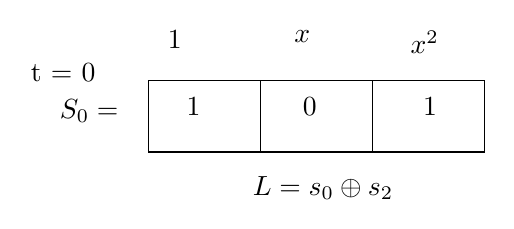
\begin{tikzpicture}[x=0.75pt,y=0.75pt,yscale=-1,xscale=1] 
        \draw   (255,893.6) -- (309,893.6) -- (309,928.2) -- (255,928.2) -- cycle ; 
        \draw   (309,893.6) -- (363,893.6) -- (363,928.2) -- (309,928.2) -- cycle ; 
        \draw   (363,893.6) -- (417,893.6) -- (417,928.2) -- (363,928.2) -- cycle ;
        
        \draw (328,900.6) node [anchor=north west][inner sep=0.75pt]   [align=left] {0};
        \draw (263,868.6) node [anchor=north west][inner sep=0.75pt]   [align=left] {1};
        \draw (324,868.6) node [anchor=north west][inner sep=0.75pt]   [align=left] {$x$};
        \draw (380,868.6) node [anchor=north west][inner sep=0.75pt]   [align=left] {$x^2$};
        \draw (197,884.6) node [anchor=north west][inner sep=0.75pt]   [align=left] {t = 0};
        \draw (211,901.6) node [anchor=north west][inner sep=0.75pt]   [align=left] {$S_0 = $};
        \draw (272,900.6) node [anchor=north west][inner sep=0.75pt]   [align=left] {1};
        \draw (386,900.6) node [anchor=north west][inner sep=0.75pt]   [align=left] {1};
        \draw (304,938.6) node [anchor=north west][inner sep=0.75pt]   [align=left] {$L = s_0 \oplus s_2$};
    \end{tikzpicture}
\end{center}
Therefore, the polynomial $g(x) = 1 + x^2$ and connecting polynomial $f(x) = x^3 + x + 1$.\\
    $1 \times g(x) = 1 + x^2$\\
    $x \times g(x) = x + x^3 = 1$\\
    $x^2 \times g(x) = x$\\
    $x^3 \times g(x) = x^2$\\
    $x^4 \times g(x) = x^3 = x + 1$\\
    $x^5 \times g(x) = x^2 + x$\\
    $x^6 \times g(x) = x^3 + x^2 = x^2 + x + 1$\\
    $x^7 \times g(x) = x^3 + x^2 + x = x + 1 + x^2 + x = 1 + x^2 = g(x)$\\
Since, after multiplication from $x^7$, g(x) is repeated again and $7 = 2^3 - 1$. Therefore, the given LFSR is fully periodic LFSR.\\


Let us now talk about the security of LFSR. Usually, we keep the secret key in the memory of LFSR, that is, in the register.

\begin{center}
    \tikzset{every picture/.style={line width=0.75pt}} 
    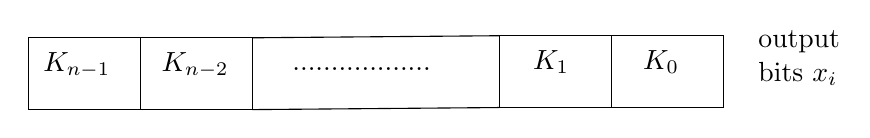
\begin{tikzpicture}[x=0.75pt,y=0.75pt,yscale=-1,xscale=1]
        \draw   (112,35) -- (166,35) -- (166,69.6) -- (112,69.6) -- cycle ; 
        \draw   (166,35) -- (220,35) -- (220,69.6) -- (166,69.6) -- cycle ;
        \draw   (339,34) -- (393,34) -- (393,68.6) -- (339,68.6) -- cycle ;
        \draw   (393,34) -- (447,34) -- (447,68.6) -- (393,68.6) -- cycle ;
        \draw    (220,69.6) -- (339,68.6) ;
        \draw    (220,35) -- (339,34) ;
        
        \draw (118,41) node [anchor=north west][inner sep=0.75pt]   [align=left] {$K_{n-1}$};
        \draw (175,41) node [anchor=north west][inner sep=0.75pt]   [align=left] {$K_{n-2}$};
        \draw (238,48) node [anchor=north west][inner sep=0.75pt]   [align=left] {..................};
        \draw (354,40) node [anchor=north west][inner sep=0.75pt]   [align=left] {$K_1$};
        \draw (407,40) node [anchor=north west][inner sep=0.75pt]   [align=left] {$K_0$};
        \draw (462.55,30.39) node [anchor=north west][inner sep=0.75pt]   [align=left] {output\\bits $x_i$};
    \end{tikzpicture}

    $K = K_0K_1.....K_{n-1}$
\end{center}

We will keep secret key or some other public parameter in the register and we will generate some bits.
\begin{center}
    output bits $x_i \rightarrow$ keystream bits $Z_i$\\
    $m_i \oplus Z_i = C_i \rightarrow$ ciphertext bits
\end{center}

Every time we will be clocking the LFSR, we will get one bit as output and will have feedback also. Now, if we consider Known Plaintext Attack Model, that is, we know certain plaintext bits and corresponding ciphertext bits and our aim is to find the secret key. Therefore, we know $m_i$ and $c_i$. Clearly,
\begin{center}
    $Z_i = m_i \oplus C_i$
\end{center}
Therefore, we know $Z_i$ corresponding to the know $m_i$ and $C_i$. Now, first output bit according to LFSR id $K_0$, the second output bit is $K_1$ and so on. That is, if we know the first n bits of the message and corresponding ciphertext, we can get entire secret key.\\
\newline
Even if we don't know the first n keystream bits, we can form a linear system of equations, because whatever bit we will get at leftmost position during clocking will be a linear function on the initial state only. For example, in the first clocking, 
\begin{center}
    $K_n = L(K_0, K_1,....., K_{n-1})$
\end{center}
and in the second clocking,
\begin{center}
    $K_{n+1} = L(K_1, K_2,....., K_n)$
\end{center}
but $K_n$ in again a linear combination of initial state only. Eventually, every bit coming to leftmost position is linear function on initial state only. Therfore, even if we know any key stream bits, that is any message bit and corresponding ciphertext bit, then,
\begin{center}
    $Z_i = m_i \oplus C_i$
\end{center}
and $Z_i$ will always be a linear function of $K_0, K_1,....., K_{n-1}$. If we know first n bits, $Z_i$ is a linear function with only one term ($K_0$ or $K_1$ or $K_{n-1}$). So, if we know $Z_i$ from known plaintext attack for any message bits. It is not required to know consecutive first n-bits. If we know any mesage bits and corresponding ciphertext bits, we can form a system of linear equations and solve that to get the secret key. Hence, simple LFSR does not provide good security.\\
\newline
Let us say you know one bit of message and corresponding ciphertext, that means you have only one linear equation. Let us say some $i^{th}$ bit (that is, not necessarily the first bit). Is is possible to reduce the search complexity of the secret key using that equation. The exhaustive search complexity of recovering the secret key is $2^n$ because this many keys are possible.\\
\newline
Let us say there is one $Z_i = 0$ and the linear equation formed is,
\begin{center}
    $Z_i = L(K_0, K_1,....., K_{n-1})$\\
    $0 = Z_i = K_2 \oplus K_6 \oplus K_{n-2}$\\
\end{center}
Using the linear equation, is it possible to reduce the complexity of searching the key? If we have correct guess for say $K_6$ and $K_{n-2}$, then $K_2$ is always determined. The search complexity, thus, is reduced to half.\\
Therefore, depending upon how many equations you are getting and the property of the system of equations, the search complexity will be reduced definitely. Therefore, knowing only 1 bit creates huge impact on the search complexity.\\
Say we have one system of linear equations with infinite solutions, so we will get all possible solutions here. So, if we have n variables but we have only few equations (say 5 or 6), still these equations will reduce the search complexity by a good margin. Therefore, using Known Plaintext Attack it is easy to break LFSR.\\

\subsubsection*{LFSR with Non-Linear Filter Function}
Here, we will consider an l-bit boolean function $f$ which takes l-bits as input and produces one bit as output. We will take l-bits out of the n-bits of the state of LFSR as input to f and use the output of $f$ as $Z_i \in \{0, 1\}$. The function $f$ here is a non-linear function.
\begin{center}
    \tikzset{every picture/.style={line width=0.75pt}}        
    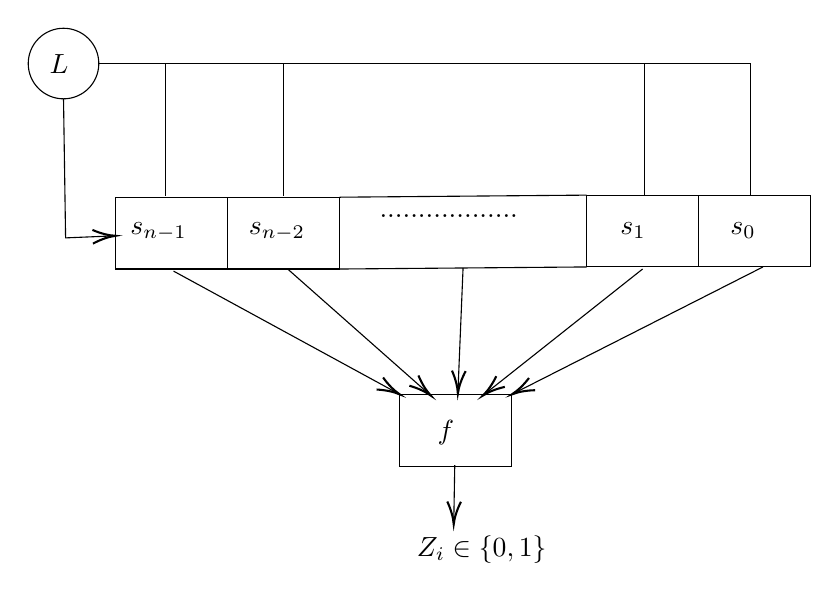
\begin{tikzpicture}[x=0.75pt,y=0.75pt,yscale=-1,xscale=1]
        \draw   (138,1067.4) -- (192,1067.4) -- (192,1102) -- (138,1102) -- cycle ;
        \draw   (192,1067.4) -- (246,1067.4) -- (246,1102) -- (192,1102) -- cycle ;
        \draw   (365,1066.4) -- (419,1066.4) -- (419,1101) -- (365,1101) -- cycle ;
        \draw    (246,1067.4) -- (365,1066.4) ;
        \draw   (419,1066.4) -- (473,1066.4) -- (473,1101) -- (419,1101) -- cycle ; 
        \draw    (246,1102) -- (365,1101) ;
        \draw    (166,1103) -- (273.24,1161.44) ;
        \draw [shift={(275,1162.4)}, rotate = 208.59] [color={rgb, 255:red, 0; green, 0; blue, 0 }  ][line width=0.75]    (10.93,-3.29) .. controls (6.95,-1.4) and (3.31,-0.3) .. (0,0) .. controls (3.31,0.3) and (6.95,1.4) .. (10.93,3.29)   ; 
        \draw    (130,1003) -- (444,1003) -- (444,1066.4) ;
        \draw   (96,1003) .. controls (96,993.61) and (103.61,986) .. (113,986) .. controls (122.39,986) and (130,993.61) .. (130,1003) .. controls (130,1012.39) and (122.39,1020) .. (113,1020) .. controls (103.61,1020) and (96,1012.39) .. (96,1003) -- cycle ;
        \draw    (113,1020) -- (114,1087) -- (136,1086.08) ;
        \draw [shift={(138,1086)}, rotate = 177.61] [color={rgb, 255:red, 0; green, 0; blue, 0 }  ][line width=0.75]    (10.93,-3.29) .. controls (6.95,-1.4) and (3.31,-0.3) .. (0,0) .. controls (3.31,0.3) and (6.95,1.4) .. (10.93,3.29)   ;
        \draw    (162,1003) -- (162,1067) ;
        \draw    (219,1003) -- (219,1067) ; 
        \draw    (393,1003) -- (393,1067) ; 
        \draw   (275,1162.4) -- (329,1162.4) -- (329,1197) -- (275,1197) -- cycle ; 
        \draw    (221,1102) -- (288.5,1161.68) ;
        \draw [shift={(290,1163)}, rotate = 221.48] [color={rgb, 255:red, 0; green, 0; blue, 0 }  ][line width=0.75]    (10.93,-3.29) .. controls (6.95,-1.4) and (3.31,-0.3) .. (0,0) .. controls (3.31,0.3) and (6.95,1.4) .. (10.93,3.29)   ;
        \draw    (392,1102) -- (316.57,1161.76) ;
        \draw [shift={(315,1163)}, rotate = 321.61] [color={rgb, 255:red, 0; green, 0; blue, 0 }  ][line width=0.75]    (10.93,-3.29) .. controls (6.95,-1.4) and (3.31,-0.3) .. (0,0) .. controls (3.31,0.3) and (6.95,1.4) .. (10.93,3.29)   ;
        \draw    (450,1101) -- (330.78,1161.49) ;
        \draw [shift={(329,1162.4)}, rotate = 333.1] [color={rgb, 255:red, 0; green, 0; blue, 0 }  ][line width=0.75]    (10.93,-3.29) .. controls (6.95,-1.4) and (3.31,-0.3) .. (0,0) .. controls (3.31,0.3) and (6.95,1.4) .. (10.93,3.29)   ;
        \draw    (305.5,1101.5) -- (303.08,1160) ;
        \draw [shift={(303,1162)}, rotate = 272.37] [color={rgb, 255:red, 0; green, 0; blue, 0 }  ][line width=0.75]    (10.93,-3.29) .. controls (6.95,-1.4) and (3.31,-0.3) .. (0,0) .. controls (3.31,0.3) and (6.95,1.4) .. (10.93,3.29)   ;
        \draw    (301.5,1196.5) -- (301.04,1223) ;
        \draw [shift={(301,1225)}, rotate = 271.01] [color={rgb, 255:red, 0; green, 0; blue, 0 }  ][line width=0.75]    (10.93,-3.29) .. controls (6.95,-1.4) and (3.31,-0.3) .. (0,0) .. controls (3.31,0.3) and (6.95,1.4) .. (10.93,3.29)   ;
        
        \draw (144,1078.4) node [anchor=north west][inner sep=0.75pt]   [align=left] {$s_{n-1}$};
        \draw (201,1078.4) node [anchor=north west][inner sep=0.75pt]   [align=left] {$s_{n-2}$};
        \draw (264,1074.4) node [anchor=north west][inner sep=0.75pt]   [align=left] {..................};
        \draw (380,1078.4) node [anchor=north west][inner sep=0.75pt]   [align=left] {$s_1$};
        \draw (433,1078.4) node [anchor=north west][inner sep=0.75pt]   [align=left] {$s_0$};
        \draw (105,997.4) node [anchor=north west][inner sep=0.75pt]   [align=left] {$L$};
        \draw (282,1229.4) node [anchor=north west][inner sep=0.75pt]   [align=left] {$Z_i \in \{0,1\}$};
        \draw (292,1173.4) node [anchor=north west][inner sep=0.75pt]   [align=left] {$f$};
    \end{tikzpicture}\\
    \vspace{2mm}
    $f: \{0, 1\}^l \rightarrow \{0, 1\}$\\
    \vspace{1mm}
    $n \geq l$\\
    \vspace{1mm}
    $C_i = m_i \oplus Z_i$
\end{center}

The state update function of LFSR will be same - there will be linear feedback function (L) and shifting as earlier. Therefore, if we select $l$ fixed position from the $n$ positions in the register, at each clocking the value at these position will update. If the function $f$ is good enough, the output will still be random looking. In fact, this will also have full period if $f$ is a good function and the connection polynomial corresponding to $L$ is primitive.\\
\newline
The advantage here is that even if we know $m_i$ and corresponding $c_i$ from Known Plaintext Attack model, and consequently we know $Z_i$. The $Z_i$ is now a non-linear function of state bits of LFSR. Solving a non-linear system of equation might be computationally difficult.\\
\newline
The state update function of LFSR is, say $\alpha$. Therefore, 
\begin{center}
    $S_{t+1} = \alpha(S_t)$\\
    $Z_{t+1} = f(S_{t+1})$
\end{center}
Let us look at the LFSR state at clocking time t.
\begin{center}
    $S_t = (s_{n-1}^t, s_{n-2}^t,....., s_0^t)$
\end{center}
The state of LFSR at clocking time (t+1) will be, 
\begin{center}
    $S_{t+1} = (s_{n-1}^{t+1}, s_{n-2}^{t+1},....., s_0^{t+1})$
\end{center}
Suppose the shifting to be right shift, therefore, 
\begin{center}
    $s_0^{t+1} = s_1^t, s_1^{t+1} = s_2^t,....,s_{n-2}^{t+1} = s_{n-1}^t, s_{n-1}^{t+1} = L(s_{n-1}^t, s_{n-2}^t,....., s_0^t)$
\end{center}
The state update can be represented as a matrix multiplication in the following way,
\begin{center}
    $ S^{t+1} = 
    \begin{bmatrix}
        s_0^{t+1}\\
        s_1^{t+1}\\
        \vdots\\
        S_{n-1}^{t+1}\\
    \end{bmatrix}
    =
    \begin{bmatrix}
        0 & 1 & 0 & 0 & \hdots & 0\\
        0 & 0 & 1 & 0 & \hdots & 0\\
        0 & 0 & 0 & 1 & \hdots & 0\\
        \vdots & \vdots & \vdots & \vdots & \ddots & \vdots\\
        0 & 0 & 0 & 0 & \hdots & 1\\
        c_n & c_{n-1} & c_{n-2} & c_{n-3} & \hdots & c_1\\
    \end{bmatrix}
    \begin{bmatrix}
        s_0^{t}\\
        s_1^{t}\\
        \vdots\\
        S_{n-1}^{t}\\
    \end{bmatrix}
    $\\
    \vspace{2mm}
    $L = c_n\cdot s_0 \oplus c_{n-1} \cdot s_1 \oplus \hdots \oplus c_1\cdot s_{n-1}$
\end{center}

\subsubsection*{LFSR with Combiner Function}
We have a similar function $f$ as we discussed above. However, here we have $l$ number of LFSR's. The output of these $l$ LFSR's, that is, l-bits becomes the input for the combiner function $f$ whose output is treated as $Z_i$. The function $f$ is non-linear.

\begin{center}
    \tikzset{every picture/.style={line width=0.75pt}}
    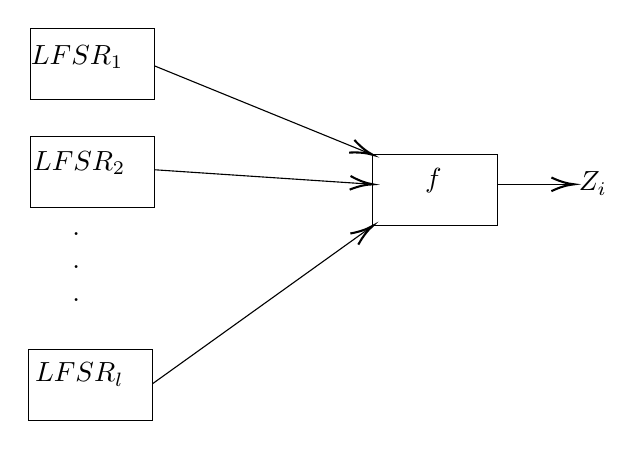
\begin{tikzpicture}[x=0.75pt,y=0.75pt,yscale=-1,xscale=1]
        \draw   (121,47) -- (181,47) -- (181,81.2) -- (121,81.2) -- cycle ;
        \draw   (120,202) -- (180,202) -- (180,236.2) -- (120,236.2) -- cycle ;
        \draw   (121,99) -- (181,99) -- (181,133.2) -- (121,133.2) -- cycle ;
        \draw   (286,108) -- (346,108) -- (346,142.2) -- (286,142.2) -- cycle ;
        \draw    (181,65.2) -- (284.15,107.25) ;
        \draw [shift={(286,108)}, rotate = 202.18] [color={rgb, 255:red, 0; green, 0; blue, 0 }  ][line width=0.75]    (10.93,-3.29) .. controls (6.95,-1.4) and (3.31,-0.3) .. (0,0) .. controls (3.31,0.3) and (6.95,1.4) .. (10.93,3.29)   ;
        \draw    (181,115.2) -- (284,122.07) ;
        \draw [shift={(286,122.2)}, rotate = 183.81] [color={rgb, 255:red, 0; green, 0; blue, 0 }  ][line width=0.75]    (10.93,-3.29) .. controls (6.95,-1.4) and (3.31,-0.3) .. (0,0) .. controls (3.31,0.3) and (6.95,1.4) .. (10.93,3.29)   ;
        \draw    (180,218.2) -- (284.37,143.37) ;
        \draw [shift={(286,142.2)}, rotate = 144.36] [color={rgb, 255:red, 0; green, 0; blue, 0 }  ][line width=0.75]    (10.93,-3.29) .. controls (6.95,-1.4) and (3.31,-0.3) .. (0,0) .. controls (3.31,0.3) and (6.95,1.4) .. (10.93,3.29)   ;
        \draw    (346,122.2) -- (381,122.2) ;
        \draw [shift={(383,122.2)}, rotate = 180] [color={rgb, 255:red, 0; green, 0; blue, 0 }  ][line width=0.75]    (10.93,-3.29) .. controls (6.95,-1.4) and (3.31,-0.3) .. (0,0) .. controls (3.31,0.3) and (6.95,1.4) .. (10.93,3.29)   ;
        
        \draw (120,54) node [anchor=north west][inner sep=0.75pt]   [align=left] {$LFSR_1$};
        \draw (121,105) node [anchor=north west][inner sep=0.75pt]   [align=left] {$LFSR_2$};
        \draw (122,207) node [anchor=north west][inner sep=0.75pt]   [align=left] {$LFSR_l$};
        \draw (310,113) node [anchor=north west][inner sep=0.75pt]   [align=left] {$f$};
        \draw (140,144) node [anchor=north west][inner sep=0.75pt]   [align=left] {.\\.\\.};
        \draw (384,115) node [anchor=north west][inner sep=0.75pt]   [align=left] {$Z_i$};
    \end{tikzpicture}\\
    $C_i = m_i \oplus Z_i$
\end{center}    

\subsection*{Non-Linear Feedback Shift Register}
After a few years, it was observed that LFSRs are good ciphers which are still secure but most of the ciphers can be broken using various adverse cryptanalysis techniques.\\
\newline
To prevent all this, there is a concept of stream ciphers known as Non-Linear Feedback Shift Register (NFSR's). From the name, it can be anticipated that the feedback function will be non-linear in NFSR. In fact, in modern scenarios, all stream ciphers are based on NFSR.\\
\newline
In NFSR, the mechanism is similar to LFSR, but the feedback is non-linear. \\
\textbf{Note: } The problem in NFSR is that if we consider a Non-Linear Feedback Function, there is no methodical proof which can determine the period of NFSR. For LFSR, if the connection polynomial is primitive, then the LFSR is fully periodic. In case of NFSR, we don't have any such proof or method.

\section*{Hash Function:}
\begin{center}
    $h: A \to B$
\end{center}
$h(x) = Y$ 
\begin{enumerate}
    \item If x is altered to $\acute{x}$ then $h(\acute{x})$ will be completely different from $h(x)$
    \item Given Y it is practically infeasible to find x such that $h(x) = Y$
    \item Given x and $Y = h(x)$ practically infeasible to find $\acute{x}$ such that $h(x) = h(\acute{x})$
\end{enumerate}
\begin{itemize} 
\item 
\begin{center}
    Alice $\longleftrightarrow$ Bob \\
    $x = E(M,k) \longrightarrow x_1 = Dec(\tilde{x}, k)$ \\
    $s_1 = h(M,k) \longrightarrow s_2$
\end{center}
If $h(x,k) = s_2$, then Bob would accept $x_1$ \\
We will be able to verify:
\begin{enumerate}
    \item Whether x is altered during communication.
    \item Whether $s_1$ is altered during communication.
\end{enumerate}
\item \textbf{Definition:}\\
A hash family is a four tuple $(P, S, K, H)$ satisfying:
\begin{enumerate}
    \item P is the set of all possible messages.
    \item S is the set of all possible message digests or authentication tags.
    \item K is the key space.
    \item For each $K_1 \in K$ there is a hash function $h_{k_1} \in H$ such that \\
    $h_{k_1}: P \to S$
\end{enumerate}
Here $|P| \ge |S|$\\
more interestingly $|P| \ge 2x|S|$ \\\\
\tikzset{every picture/.style={line width=0.75pt}} %set default line width to 0.75pt        

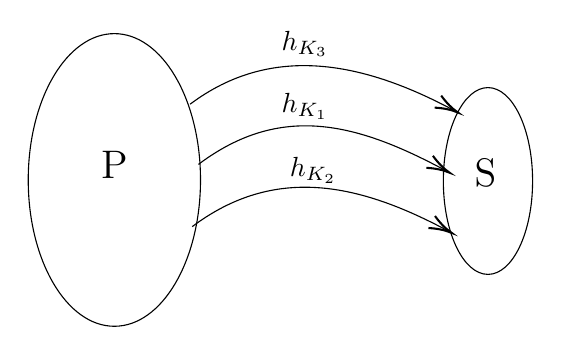
\begin{tikzpicture}[x=0.75pt,y=0.75pt,yscale=-1,xscale=1]
%uncomment if require: \path (0,300); %set diagram left start at 0, and has height of 300

%Shape: Ellipse [id:dp6385929644721748] 
\draw   (130.2,139.1) .. controls (130.2,100.16) and (148.78,68.6) .. (171.7,68.6) .. controls (194.62,68.6) and (213.2,100.16) .. (213.2,139.1) .. controls (213.2,178.04) and (194.62,209.6) .. (171.7,209.6) .. controls (148.78,209.6) and (130.2,178.04) .. (130.2,139.1) -- cycle ;
%Shape: Ellipse [id:dp35632658610404433] 
\draw   (330.2,139.6) .. controls (330.2,114.75) and (339.83,94.6) .. (351.7,94.6) .. controls (363.57,94.6) and (373.2,114.75) .. (373.2,139.6) .. controls (373.2,164.45) and (363.57,184.6) .. (351.7,184.6) .. controls (339.83,184.6) and (330.2,164.45) .. (330.2,139.6) -- cycle ;
%Curve Lines [id:da9831191387685083] 
\draw    (208.2,102.6) .. controls (247.8,72.9) and (292.3,82.4) .. (335.88,105.88) ;
\draw [shift={(337.2,106.6)}, rotate = 208.61] [color={rgb, 255:red, 0; green, 0; blue, 0 }  ][line width=0.75]    (10.93,-3.29) .. controls (6.95,-1.4) and (3.31,-0.3) .. (0,0) .. controls (3.31,0.3) and (6.95,1.4) .. (10.93,3.29)   ;
%Curve Lines [id:da7449905549695661] 
\draw    (212.2,131.6) .. controls (251.8,101.9) and (288.46,111.4) .. (331.88,134.88) ;
\draw [shift={(333.2,135.6)}, rotate = 208.61] [color={rgb, 255:red, 0; green, 0; blue, 0 }  ][line width=0.75]    (10.93,-3.29) .. controls (6.95,-1.4) and (3.31,-0.3) .. (0,0) .. controls (3.31,0.3) and (6.95,1.4) .. (10.93,3.29)   ;
%Curve Lines [id:da6241272700976574] 
\draw    (209.2,161.6) .. controls (248.8,131.9) and (289.38,140.42) .. (332.88,163.88) ;
\draw [shift={(334.2,164.6)}, rotate = 208.61] [color={rgb, 255:red, 0; green, 0; blue, 0 }  ][line width=0.75]    (10.93,-3.29) .. controls (6.95,-1.4) and (3.31,-0.3) .. (0,0) .. controls (3.31,0.3) and (6.95,1.4) .. (10.93,3.29)   ;

% Text Node
\draw (164,124) node [anchor=north west][inner sep=0.75pt]   [align=left] {{\Large P}};
% Text Node
\draw (344,128) node [anchor=north west][inner sep=0.75pt]   [align=left] {{\Large S}};
% Text Node
\draw (251,66) node [anchor=north west][inner sep=0.75pt]   [align=left] {$h_{K_3}$};
% Text Node
\draw (251,96) node [anchor=north west][inner sep=0.75pt]   [align=left] {$h_{K_1}$};
% Text Node
\draw (255,127) node [anchor=north west][inner sep=0.75pt]   [align=left] {$h_{K_2}$};


\end{tikzpicture}

Where H : set of all hash function
$h_{k_i}$ : hash function
\end{center}
where H is the set of all hash functions and $h_{k_i}$ is the hash function
\item If the key is involved in the computation of hashed value, then that hash function is known as \textbf{keyed hash function}.\\\\
If the key is not required to compute the hashed value then that hash function is known as \textbf{unkeyed hash function}.
\end{itemize}
\section*{Problems:}
\begin{itemize}
    \item \textbf{Problem 1: Pre-Image Finding} \\
    $h: P \to S$ \\
    \begin{itemize}
        \item Given $y \in S$, Find $x \in P$ such that $h(x) = y$.\\
    \end{itemize}
This problem is known as pre-image finding problem.\\\\
For an hash function h, if you cannot find pre-image in a feasible time then h is known as pre-image resistant hash function.
\begin{itemize}
    \item Finding pre-image is computationally hard for pre-image resistant hash function.
\end{itemize}
\item \textbf{Problem 2: Second Pre-Image Finding}\\
$h: P \to S$\\
\begin{itemize}
    \item Given $x \in P$ and $h(x)$ find $\acute{x} \in P$ such that $\acute{x} \ne x$ and $h(\acute{x}) = h(x)$\\
\end{itemize}
This problem is known as second pre-image finding problem.\\\\
If finding second pre-image is computationally hard for h then, h is known as second pre-image resistant hash function.
\item \textbf{Problem 3: Collision Finding Problem}\\
$h: P \to S$\\\\
\begin{itemize}
    \item Find $x, \acute{x} \in P$ such that $\acute{x} \ne x$ and $h(x) = h(\acute{x})$.\\
\end{itemize}
This problem is known as collision finding problem.\\
For an hash function h if finding collision is computationally hard then h is known as collision resistant hash function.
\end{itemize}
\subsection*{Ideal Hash Function:}
Consider a hash function $h: P \to S$.\\\\
h will be called ideal hash function if given $x \in P$ to find $h(x)$ either you have to apply h on x or you have to look into the total corresponding to h(hash table).
\section*{Pre-Image Finding Algorithm:}
\textbf{Question:} Given $y \in Y$, find $x \in X$ such that $h(x) = y$
$h: X \to Y$\\\\
Choose any $x_0 \subseteq x$ such that $|x_0| = Q$ for each $x \in x_0$\\\\
Compute $y_x = h(x)$\\
if $y_x = y$\\
return x\\\\
$x_0 = \{ x_1, x_2, \dots, x_Q \}$\\
$E_i:$ event $h(x_i) = y; 1 \le i \le Q$\\\\
$P_r[E_i] = \frac{1}{M}$\\\\
$P_r[{E_i}^c] = 1 - \frac{1}{M}$\\\\
$P_r[E_1 \cup E_2 \cup E_3 \cup \dots \cup E_Q]$\\\\
$= 1 - P_r[{E_1}^c \cup {E_2}^c \cup {E_3}^c \cup \dots \cup {E_Q}^c]$\\\\
$= 1 - \prod_{i = 1}^{Q} P_r[{E_i}^c]$\\\\
$= 1 - {(1- \frac{1}{M})}^Q$\\\\
$= 1 - [1 - ({Q \atop 1})\frac{1}{M} + ({Q \atop 2})\frac{1}{M^2} - \dots]$\\\\
$\simeq 1 - [1 - ({Q \atop 1})\frac{1}{M}]$\\\\
$= \frac{Q}{M}$\\\\
$P_r$[Pre-image finding] $\simeq \frac{Q}{M}$\\\\
Complexity of finding pre-image = $O(M)$.









\end{document}